\chapter{Architettura Software}
\label{chap:architettura_software}

La traduzione del rigoroso ecosistema matematico descritto nel capitolo precedente in un ambiente virtuale interattivo richiede una solida base informatica. Questo capitolo analizza l'architettura Object-Oriented (OOP) sviluppata all'interno del motore grafico Unreal Engine 5, illustrando come le entità fisiche della simulazione siano state modellate attraverso classi C++ specializzate, garantendo sia prestazioni in tempo reale sia fedeltà numerica nell'integrazione astrodinamica.

%%%%%%%%%%%%%%%%%%%%%%%%%%%%%%%%%%%%%%%%%%%%%%%%%%%%%%%%%%%%%%%%%%%%%%%%%%%%%%%%%%%%%%%%%%%%%%%%%%%%%
%%%%%%%%%%%%%%%%%%%%%%%%%%%%%%%%%%%%%%%%%%%%%%%%%%%%%%%%%%%%%%%%%%%%%%%%%%%%%%%%%%%%%%%%%%%%%%%%%%%%%

\section{Unreal Engine come framework di calcolo scientifico}
L'utilizzo di un motore grafico commerciale per scopi di ricerca astrodinamica richiede un parziale cambio di paradigma rispetto all'uso tradizionale orientato all'intrattenimento. In questo elaborato, Unreal Engine non viene impiegato per le sue capacità puramente estetiche, ma viene trattato come un vero e proprio \textit{framework} di calcolo scientifico \cite{ericson2004real}. 

Sfruttando il suo nucleo nativo in C++ ad alte prestazioni, il motore fornisce un'infrastruttura robusta per l'esecuzione di calcoli vettoriali complessi, la gestione spaziale tridimensionale e l'aggiornamento temporale continuo delle variabili cinematiche. Per comprendere come il modello matematico della vela solare sia stato tradotto in codice eseguibile, è imperativo analizzare i due pilastri architetturali su cui si fonda Unreal Engine: il modello compositivo e la gestione discreta del tempo.

%%%%%%%%%%%%%%%%%%%%%%%%%%%%%%%%%%%%%%%%%%%%%%%%%%%%%%%%%%%%%%%%%%%%%%%%%%%%%%%%%%%%%%%%%%%%%%%%%%%%%

\subsection{Il paradigma Actor-Component}
A differenza della classica programmazione orientata agli oggetti basata su un'ereditarietà profonda e monolitica, l'architettura di Unreal Engine predilige fortemente la composizione rispetto all'ereditarietà. Questo approccio altamente modulare si concretizza nel paradigma \textit{Actor-Component}.

All'interno del motore, l'entità fondamentale in grado di esistere nello spazio tridimensionale è definita dalla classe base \lstinline|AActor|. Un Attore, di per sé, è un contenitore astratto provvisto di una trasformazione spaziale globale (posizione, rotazione e scala vettoriale), ma intrinsecamente privo di logica fisica o rappresentazione visiva. Per dotare un Attore di comportamenti tangibili, l'ingegnere del software deve "assemblare" al suo interno diverse istanze derivate dalla classe \lstinline|UActorComponent|. 



Nel contesto del simulatore sviluppato, il veicolo spaziale principale (\lstinline|ASolarSail|) è stato progettato istanziando e combinando strategicamente componenti specifici:
\begin{itemize}
    \item \textbf{Componenti strutturali:} Un \lstinline|UStaticMeshComponent| viene utilizzato per definire la geometria esatta della membrana della vela. Oltre a fornire la rappresentazione visiva, questo componente genera il \textit{collider} matematico necessario agli algoritmi di \textit{ray casting} per determinare dinamicamente l'area esposta al flusso fotonico.
    \item \textbf{Componenti logici e direzionali:} Componenti specializzati, come l'\lstinline|UArrowComponent|, vengono ancorati all'Attore per rappresentare visivamente e computazionalmente i sistemi di riferimento locali (come il versore normale $\mathbf{n}$ alla superficie della vela), fondamentali per il continuo ricalcolo dell'angolo di incidenza solare ($\alpha$).
\end{itemize}

Tale rigida separazione delle responsabilità (\textit{Separation of Concerns}) rende l'architettura del simulatore estremamente flessibile. La complessa logica di integrazione orbitale risiede all'interno della classe principale dell'Attore, mentre l'onere del calcolo delle intersezioni spaziali viene delegato ai componenti geometrici sottostanti, massimizzando l'efficienza computazionale del processore.

\begin{figure}[htbp!]
    \centering
    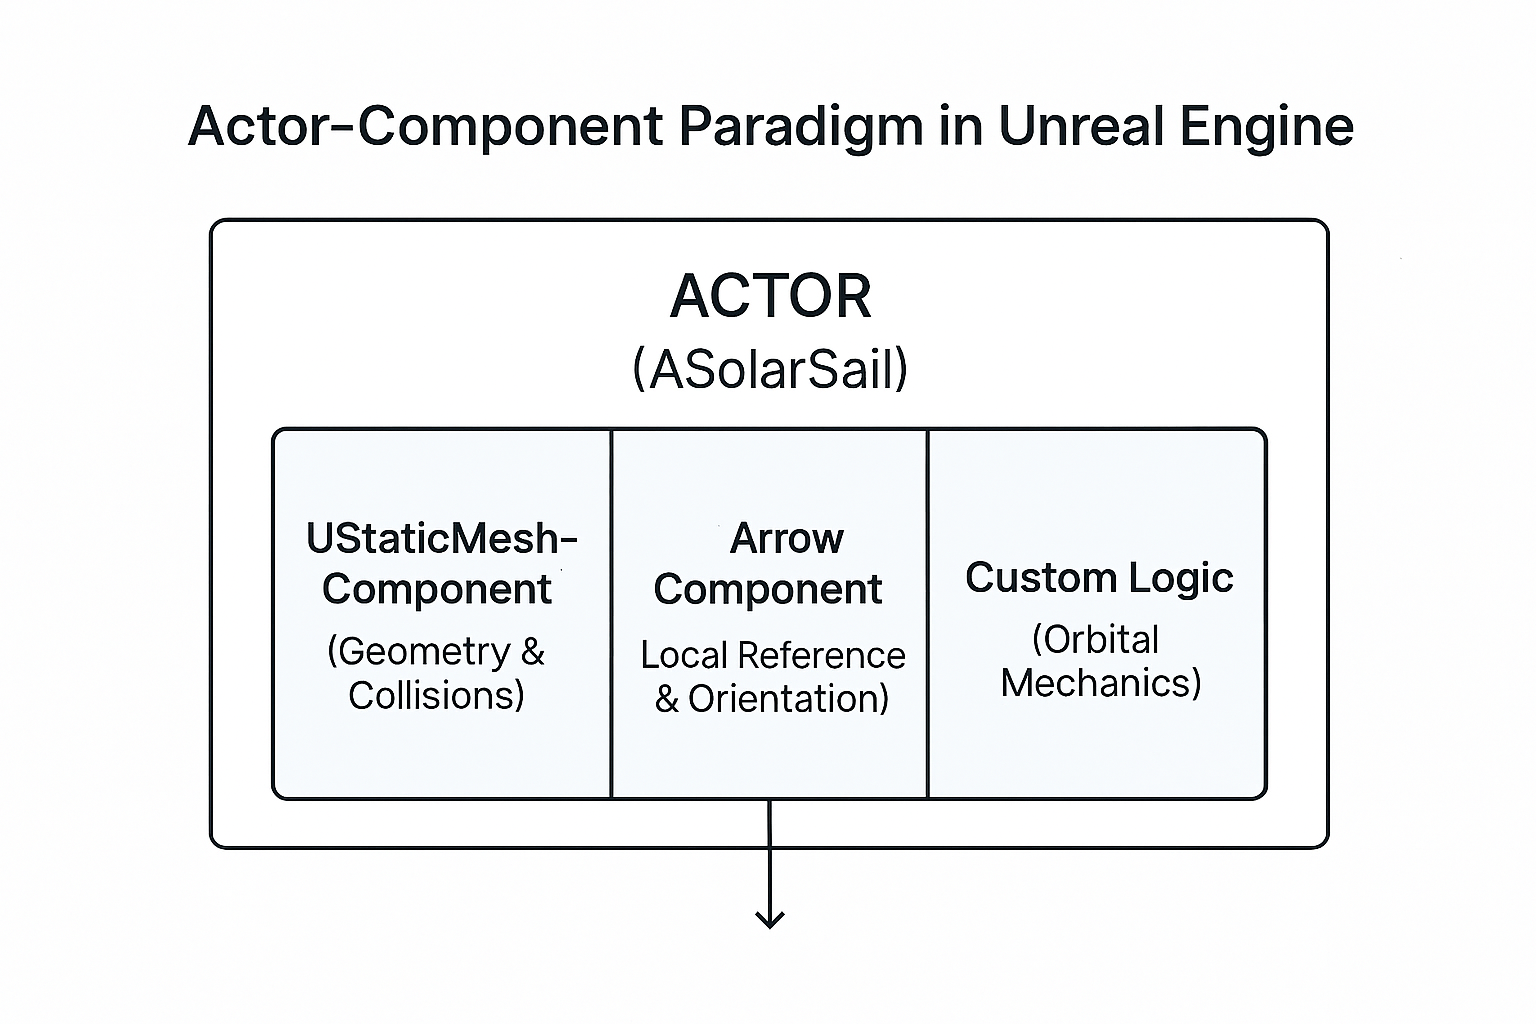
\includegraphics[width=0.75\textwidth]{Images/actor_component_diagram.png}
    \caption{Schema concettuale del paradigma Actor-Component in Unreal Engine: un singolo Attore funge da contenitore per logica, geometria e collisioni.}
    \label{fig:actor_component}
\end{figure}

%%%%%%%%%%%%%%%%%%%%%%%%%%%%%%%%%%%%%%%%%%%%%%%%%%%%%%%%%%%%%%%%%%%%%%%%%%%%%%%%%%%%%%%%%%%%%%%%%%%%%

\subsection{Il ciclo di vita degli oggetti e il sistema di Tick}
Il secondo elemento cruciale per la simulazione di sistemi dinamici è la discretizzazione e la gestione del tempo informatico. All'interno di Unreal Engine, il ciclo di vita di ogni Attore è scandito da metodi virtuali specifici che il programmatore può sovrascrivere (\textit{override}) in C++ per iniettare la logica matematica desiderata. I due metodi cardine su cui si basa l'integrazione numerica dell'intero simulatore sono \lstinline|BeginPlay()| e \lstinline|Tick()|.

L'inizializzazione del modello fisico avviene all'interno della funzione \lstinline|BeginPlay()|. Invocata una singola volta nell'esatto momento in cui l'Attore viene generato nello spazio (o al lancio della simulazione), questa funzione è deputata all'allocazione delle risorse di memoria, alla definizione delle masse strutturali a secco e, nel caso della vela solare, al calcolo istantaneo della velocità orbitale circolare necessaria a garantire la stabilità kepleriana di partenza, calcolando visivamente l'orbita di parcheggio.

Terminata la delicata fase di inizializzazione, il controllo passa alla funzione \lstinline|Tick(float DeltaTime)|, che rappresenta il vero cuore pulsante del \textit{solver} astrodinamico. A differenza dei solutori matematici statici che calcolano traiettorie predeterminate, il motore grafico opera tramite un ciclo continuo (il \textit{game loop}). Ad ogni fotogramma (\textit{frame}) renderizzato dalla scheda video, il motore invoca la funzione \lstinline|Tick| su tutti gli Attori attivi, fornendo come parametro di ingresso il \lstinline|DeltaTime| ($\Delta t$). Tale parametro rappresenta in modo rigoroso l'intervallo temporale, espresso in frazioni di secondo, trascorso dalla precedente esecuzione.

In ottica astrodinamica, il \lstinline|DeltaTime| assume il ruolo di passo di integrazione (il $dt$ delle equazioni differenziali ordinarie). Ad ogni singola esecuzione del \lstinline|Tick|, l'Attore \lstinline|ASolarSail| esegue sequenzialmente i seguenti calcoli computazionali:
\begin{enumerate}
    \item Interroga i propri componenti geometrici per ricalcolare l'area effettiva esposta al Sole ($A_{\text{eff}}$) basandosi sull'assetto istantaneo.
    \item Calcola la risultante vettoriale delle forze in gioco, sommando l'attrazione gravitazionale ($\mathbf{a}_g$) e la pressione di radiazione solare ($\mathbf{a}_{\text{SRP}}$).
    \item Integra le forze ricavando la nuova accelerazione netta, la quale viene moltiplicata per il \lstinline|DeltaTime| per ottenere la variazione di velocità vettoriale ($d\mathbf{v}$).
    \item Aggiorna la trasformazione spaziale 3D del veicolo in base alla nuova cinematica locale.
\end{enumerate}

\begin{figure}[htbp!]
    \centering
    % 
\includegraphics[width=0.8\textwidth]{Images/tick_physics_loop.png}
    \caption{Diagramma di flusso dell'integrazione numerica eseguita a ogni ciclo di \textit{Tick}: il motore grafico funge da solutore iterativo per le equazioni differenziali del moto.}
    \label{fig:tick_physics_loop}
\end{figure}

Questo approccio a ciclo continuo garantisce che la simulazione avvenga in modo fluido e interattivo, permettendo all'ingegnere di variare a \textit{runtime} l'inclinazione della vela solare e osservare istantaneamente come tali variazioni modifichino l'accelerazione netta e la conseguente traiettoria del veicolo fotonico.

%%%%%%%%%%%%%%%%%%%%%%%%%%%%%%%%%%%%%%%%%%%%%%%%%%%%%%%%%%%%%%%%%%%%%%%%%%%%%%%%%%%%%%%%%%%%%%%%%%%%%
%%%%%%%%%%%%%%%%%%%%%%%%%%%%%%%%%%%%%%%%%%%%%%%%%%%%%%%%%%%%%%%%%%%%%%%%%%%%%%%%%%%%%%%%%%%%%%%%%%%%%

\section{Progettazione Object-Oriented (OOP) del sistema}
La validità di un simulatore scientifico non risiede unicamente nell'accuratezza matematica delle sue equazioni, ma anche nella robustezza dell'infrastruttura software che le elabora e le espone all'utente. Per gestire l'intrinseca complessità dello scambio vettoriale di quantità di moto, dell'integrazione orbitale in doppia precisione e dell'avanzamento temporale, il codice C++ alla base dell'applicativo è stato strutturato seguendo rigorosamente i principi della Programmazione Orientata agli Oggetti (OOP). 

Questo approccio formale garantisce un'elevata coesione interna ai singoli moduli informatici e un basso accoppiamento (\textit{loose coupling}) tra le classi, favorendo la stabilità del simulatore, la sua facile manutenibilità e la futura espansione del progetto verso scenari interplanetari.

%%%%%%%%%%%%%%%%%%%%%%%%%%%%%%%%%%%%%%%%%%%%%%%%%%%%%%%%%%%%%%%%%%%%%%%%%%%%%%%%%%%%%%%%%%%%%%%%%%%%%

\subsection{Gerarchia delle classi e diagramma UML}
La progettazione della gerarchia delle classi parte dall'estensione delle entità base fornite dal framework di Unreal Engine, sfruttando pesantemente il sistema di riflessione nativo (\textit{Reflection System}) del motore tramite le macro C++ \lstinline|UCLASS()| e \lstinline|GENERATED_BODY()|. La struttura architetturale è riassumibile in due rami principali di esecuzione, che comunicano tra loro esclusivamente tramite riferimenti deboli (\textit{pointers}) e interfacce ben definite.



Come illustrato nel diagramma UML del sistema, le entità fondanti del simulatore derivano direttamente dalla superclasse \lstinline|AActor|:
\begin{itemize}
    \item \lstinline|ASimulationManager|: Progettato seguendo una logica operativa affine al \textit{Singleton pattern} (in quanto deve rigorosamente esisterne una sola istanza attiva nel livello simulato), questo Attore funge da orchestratore globale. Esso detiene il controllo centralizzato del tempo di simulazione (\lstinline|TimeScale|), calcola il vettore direzionale globale dell'illuminazione solare e gestisce l'inizializzazione del \textit{Data Logging} persistente. La sua esistenza solleva i singoli veicoli spaziali dal gravoso compito di dover recuperare autonomamente informazioni ambientali condivise.
    \item \textbf{Gerarchia del Veicolo:} La complessa rappresentazione della vela solare è interamente incapsulata nella classe \lstinline|ASolarSail|. A sua volta, per garantire un'alta specializzazione logica, la classe delega calcoli specifici a componenti software dedicati (derivati da \lstinline|UActorComponent|). Ad esempio, la geometria di impatto e i materiali ottici sono gestiti da componenti strutturali, mentre le vitali variabili di stato orbitale (vettore posizione, vettore velocità, massa a secco) sono mantenute e protette all'interno dell'Attore principale.
\end{itemize}

Questa divisione netta e gerarchica permette di istanziare molteplici oggetti \lstinline|ASolarSail| simultaneamente all'interno dello stesso scenario (ad esempio, per testare vele competitive con aree geometriche o coefficienti di riflettività diversi) sotto la rigorosa supervisione centralizzata di un unico \lstinline|ASimulationManager|, garantendo la perfetta coerenza temporale dell'intero \textit{framework}.

\begin{figure}[htbp!]
    \centering
    % \includegraphics[width=0.8\textwidth]{Images/uml_class_diagram.jpg}
    \caption{Diagramma UML semplificato dell'architettura software: il Simulation Manager orchestra il tempo globale, mentre le istanze Solar Sail gestiscono la cinematica locale.}
    \label{fig:uml_diagram}
\end{figure}

%%%%%%%%%%%%%%%%%%%%%%%%%%%%%%%%%%%%%%%%%%%%%%%%%%%%%%%%%%%%%%%%%%%%%%%%%%%%%%%%%%%%%%%%%%%%%%%%%%%%%

\subsection{Incapsulamento dei moduli fisici e disaccoppiamento}
Il principio informatico dell'incapsulamento è stato applicato in modo stringente durante tutto lo sviluppo per proteggere l'integrità dei dati fisici e prevenire l'insorgere di stati del sistema matematicamente incoerenti (come masse strutturali negative o coefficienti ottici sommati superiori a 1, che violerebbero la conservazione dell'energia). 

Le variabili di stato cruciali per l'integrazione differenziale sono esplicitamente dichiarate con modificatori di accesso \lstinline|private| o \lstinline|protected| all'interno degli \textit{header file} (\lstinline|.h|). L'accesso e la mutazione di tali variabili dall'esterno avvengono esclusivamente tramite metodi \textit{getter} e \textit{setter} specifici. Ad esempio, la richiesta utente di modifica dell'assetto o dell'area della vela durante l'esecuzione invoca automaticamente una routine di validazione interna che ricalcola istantaneamente l'area effettiva esposta ($A_{\text{eff}}$), garantendo che la fisica vettoriale del \lstinline|Tick| non operi mai su dati obsoleti o asincroni.

Un aspetto peculiare dell'incapsulamento in ambiente Unreal Engine è l'uso strategico della macro di serializzazione \lstinline|UPROPERTY|. Per permettere all'utente finale (l'ingegnere aerospaziale o l'operatore di missione) di configurare i parametri iniziali senza dover ricompilare il codice sorgente C++, le variabili chiave sono state esposte all'editor visivo tramite specificatori mirati:

\begin{lstlisting}[language=C++, caption={Esempio di incapsulamento ed esposizione sicura dei parametri fisici in C++}]
UPROPERTY(EditAnywhere, BlueprintReadWrite, Category="Solar Sail|Physics", 
          meta=(ClampMin="0.01", UIMin="0.01"))
double DryMass;

UPROPERTY(EditAnywhere, BlueprintReadWrite, Category="Solar Sail|Optical", 
          meta=(ClampMin="0.0", ClampMax="1.0"))
double SpecularReflectance;
\end{lstlisting}

\begin{figure}[htbp!]
    \centering
    % 
\includegraphics[width=0.6\textwidth]{Images/uproperty_editor.png}
    \caption{L'esposizione sicura delle variabili di stato tramite \lstinline|UPROPERTY|. L'interfaccia generata automaticamente dall'editor rispetta i vincoli matematici imposti dai metadati C++, impedendo l'inserimento di valori fisicamente invalidi.}
    \label{fig:uproperty_editor}
\end{figure}

L'utilizzo dei metadati di restrizione (\lstinline|ClampMin|, \lstinline|ClampMax|) direttamente all'interno della macro rappresenta una trasposizione informatica diretta dei vincoli fisici naturali: impone a livello di editor che la massa non sia mai pari a zero (evitando disastrose divisioni per zero nel calcolo dell'accelerazione $\mathbf{a} = \mathbf{F}/m$) e costringe i coefficienti ottici nel ristretto dominio logico $[0, 1]$.

Dal punto di vista della logica di esecuzione, il modulo di calcolo orbitale puro (gravitazione universale di Newton) è stato tenuto logicamente disaccoppiato dal modulo ottico perturbativo (\textit{ray casting} e pressione di radiazione fotonica). La funzione \lstinline|Tick()| invoca questi sottomoduli in stretta sequenza, accumulando le singole forze in un vettore \lstinline|NetForce| tridimensionale globale. Questo approccio altamente modulare assicura che in futuro sia possibile implementare nuove perturbazioni astrodinamiche (ad esempio, l'effetto dell'albedo terrestre, l'attrazione gravitazionale di un terzo corpo come la Luna o l'attrito atmosferico residuo per orbite LEO bassissime) semplicemente aggiungendo una nuova funzione matematica alla \textit{pipeline} di sommatoria delle forze, senza dover in alcun modo alterare o riscrivere il delicato nucleo del risolutore cinematico principale.

%%%%%%%%%%%%%%%%%%%%%%%%%%%%%%%%%%%%%%%%%%%%%%%%%%%%%%%%%%%%%%%%%%%%%%%%%%%%%%%%%%%%%%%%%%%%%%%%%%%%%
%%%%%%%%%%%%%%%%%%%%%%%%%%%%%%%%%%%%%%%%%%%%%%%%%%%%%%%%%%%%%%%%%%%%%%%%%%%%%%%%%%%%%%%%%%%%%%%%%%%%%

\section{Il gestore della simulazione (Simulation Manager)}
Il corretto e coerente svolgimento di una simulazione astrodinamica interattiva richiede un'entità di supervisione astratta che svincoli i singoli veicoli spaziali dalla complessa gestione dell'ambiente condiviso. In ottemperanza ai rigorosi principi di progettazione modulare precedentemente descritti, questo ruolo apicale è ricoperto dalla classe \lstinline|ASimulationManager|. 

Derivata direttamente da \lstinline|AActor| per poter esistere fisicamente all'interno del mondo virtuale, questa classe agisce come \textit{hub} centrale dell'applicativo, garantendo che tutti gli elementi vettoriali dello scenario siano perfettamente sincronizzati rispetto a un unico orologio globale e a un unico sistema di riferimento ambientale condiviso.

%%%%%%%%%%%%%%%%%%%%%%%%%%%%%%%%%%%%%%%%%%%%%%%%%%%%%%%%%%%%%%%%%%%%%%%%%%%%%%%%%%%%%%%%%%%%%%%%%%%%%

\subsection{Inizializzazione e controllo dello stato globale}
Il primo e più critico compito del gestore si esplica nella primissima fase di avvio (\lstinline|BeginPlay()|). Il \lstinline|ASimulationManager| è unico responsabile della validazione dello stato iniziale del mondo tridimensionale. Attraverso le potenti librerie di sistema fornite dal motore (come la funzione \lstinline|UGameplayStatics::GetAllActorsOfClass|), il gestore acquisisce automaticamente all'avvio i puntatori di memoria a tutte le istanze di tipo \lstinline|ASolarSail| correntemente presenti nel livello, costruendo un registro dinamico e aggiornato dei veicoli attivi. 

Questa rigida centralizzazione informativa è fondamentale per due aspetti cardine della simulazione fisica:
\begin{itemize}
    \item \textbf{Gestione univoca del vettore solare:} Invece di costringere ogni singola vela a ricalcolare pesantemente la posizione spaziale della sorgente luminosa a ogni \textit{Tick}, il \textit{Manager} interroga una singola volta la luce direzionale del livello (che agisce come \textit{proxy} del Sole) ed estrae il versore di propagazione vettoriale della luce ($\mathbf{u}$). Questo singolo vettore viene poi trasmesso a cascata, in modo estremamente efficiente, a tutte le vele solari registrate, garantendo un'assoluta coerenza ottica e geometrica in tutto lo spazio simulato.
    \item \textbf{Controllo autoritativo del TimeScale:} Il gestore detiene in esclusiva la variabile globale \lstinline|TimeScale|, che rappresenta il fattore numerico di dilatazione temporale. Nelle simulazioni di meccanica orbitale a spinta continua, dove una singola manovra di innalzamento orbitale può durare mesi effettivi, eseguire il programma in rapporto 1:1 rispetto alla realtà è ingegneristicamente inefficace. Il \textit{Manager} funge da \textit{time-keeper} assoluto, inoltrando costantemente il valore di \lstinline|TimeScale| ai sottomoduli fisici per scalare matematicamente il parametro \lstinline|DeltaTime| ($\Delta t$). Ciò permette l'esecuzione fluida della modalità accelerata (\textit{Accelerated Time Mode}) a livello logico, mantenendo però rigorosamente stabile il \textit{framerate} di rendering visivo per l'utente.
\end{itemize}

Inoltre, lo stato globale gestito centralmente include l'inizializzazione dei complessi flussi di I/O (Input/Output). Il \lstinline|ASimulationManager| apre all'avvio i canali di comunicazione per il \textit{Data Logging}, preparando e formattando i file CSV necessari per la registrazione periodica e persistente della telemetria orbitale, sollevando così la singola classe \lstinline|ASolarSail| dal gravoso onere informatico della gestione del \textit{file system} del sistema operativo ospite.

%%%%%%%%%%%%%%%%%%%%%%%%%%%%%%%%%%%%%%%%%%%%%%%%%%%%%%%%%%%%%%%%%%%%%%%%%%%%%%%%%%%%%%%%%%%%%%%%%%%%%

\subsection{Gestione della telecamera e degli input utente}
Affinché il simulatore sviluppato in Unreal Engine funga da strumento di indagine e validazione utile, l'ingegnere deve poter ispezionare visivamente il veicolo spaziale in ogni istante e alterare i parametri critici della missione a \textit{runtime}. Poiché la vela solare (\lstinline|ASolarSail|) è concettualmente un oggetto passivo, sottoposto unicamente a rigide leggi fisiche esterne, dotarla direttamente di logiche informatiche per la lettura periferica della tastiera o del mouse violerebbe il fondamentale principio architetturale di singola responsabilità (\textit{Single Responsibility Principle}).

Il \lstinline|ASimulationManager| (operando talvolta in concerto con un \lstinline|APawn| specializzato ad esso collegato, configurato come \textit{Player Controller}) si interfaccia quindi in modo esclusivo con il moderno sistema di input del motore (\textit{Enhanced Input System}), traducendo le azioni fisiche dell'utente in precisi comandi vettoriali per la simulazione:
\begin{itemize}
    \item \textbf{Interazione visiva orbitale:} La telecamera di osservazione non è rozzamente ancorata alla geometria della vela, ma è sofisticatamente vincolata tramite un \lstinline|USpringArmComponent|. Questo braccio virtuale flessibile agisce da perfetto giunto sferico matematico, permettendo all'utente di orbitare visivamente attorno al veicolo (tramite complessi movimenti di \textit{pan}, \textit{tilt} e \textit{zoom}) mantenendo il centro di massa dinamico della vela esattamente al centro dello schermo (\textit{focus point}), il tutto in modo totalmente indipendente dall'enorme velocità orbitale del mezzo spaziale simulato.
    
    \item \textbf{Alterazione dinamica dell'assetto e del tempo:} Attraverso specifiche mappature dei tasti configurate nel motore, l'utente può incrementare o decrementare istantaneamente il \lstinline|TimeScale| globale per navigare rapidamente e fluidamente nel tempo di missione. Parallelamente, gli input direzionali continui vengono catturati, filtrati e applicati per variare in tempo reale gli angoli di Eulero di beccheggio (\textit{pitch}) e imbardata (\textit{yaw}) della vela solare. 
\end{itemize}



Quando l'utente richiede una variazione di assetto spaziale, il \textit{Manager} invia il comando vettoriale alla vela, la quale, al primissimo ciclo di \lstinline|Tick| utile, ricalcolerà immediatamente il nuovo vettore normale $\mathbf{n}$ locale, la nuova e ridotta area effettiva esposta $A_{\text{eff}}$ e la conseguente variazione dell'accelerazione perturbativa fotonica. Questa catena di eventi informatici garantisce una responsività immediata dell'interfaccia visiva del simulatore, senza mai compromettere la stabilità o la precisione numerica dell'integrazione differenziale in corso in background.

\begin{figure}[htbp!]
    \centering
    % \includegraphics[width=0.85\textwidth]{Images/editor_input_camera.jpg}
    \caption{Visuale dall'editor del simulatore: il sistema di telecamera basato su \textit{SpringArm} permette di ispezionare il veicolo senza interferire con la cinematica orbitale locale.}
    \label{fig:editor_camera}
\end{figure}

%%%%%%%%%%%%%%%%%%%%%%%%%%%%%%%%%%%%%%%%%%%%%%%%%%%%%%%%%%%%%%%%%%%%%%%%%%%%%%%%%%%%%%%%%%%%%%%%%%%%%
%%%%%%%%%%%%%%%%%%%%%%%%%%%%%%%%%%%%%%%%%%%%%%%%%%%%%%%%%%%%%%%%%%%%%%%%%%%%%%%%%%%%%%%%%%%%%%%%%%%%%

\section{Modellazione del veicolo spaziale (Solar Sail)}
Se il \lstinline|ASimulationManager| rappresenta indubbiamente il "cervello" ambientale e temporale del simulatore, la complessa classe \lstinline|ASolarSail| ne costituisce il vero e proprio fulcro fisico e cinematico. Progettata ingegneristicamente come una specializzazione avanzata della classe base \lstinline|AActor|, questa entità informatica funge da "gemello digitale" (\textit{digital twin}) della sonda spaziale fisica. Il suo scopo informatico è intrinsecamente duplice: fornire una rappresentazione spaziale estremamente accurata per il calcolo delle delicate intersezioni ottiche fotoniche e incapsulare lo stato dinamico vettoriale del veicolo, evolvendolo coerentemente istante per istante.

%%%%%%%%%%%%%%%%%%%%%%%%%%%%%%%%%%%%%%%%%%%%%%%%%%%%%%%%%%%%%%%%%%%%%%%%%%%%%%%%%%%%%%%%%%%%%%%%%%%%%

\subsection{Rappresentazione geometrica e mesh poligonale}
La membrana riflettente della vela solare simulata non è trattata informaticamente come una semplice astrazione matematica puntiforme o monodimensionale, bensì come un corpo fisico esteso nello spazio tridimensionale interplanetario. Per modellare con fedeltà questa vasta estensione planare, la classe \lstinline|ASolarSail| impiega al suo interno un \lstinline|UStaticMeshComponent|, il quale ospita e renderizza la geometria tridimensionale del velivolo progettata tramite software CAD.

La scelta progettuale di utilizzare una complessa mesh poligonale invece di forme primitive analitiche è strettamente legata alle stringenti necessità degli algoritmi di calcolo della Pressione di Radiazione Solare (SRP). Dal punto di vista informatico e del \textit{rendering}, l'immensa superficie riflettente è discretizzata e composta da un vasto insieme di triangoli complanari. Questa discretizzazione geometrica avanzata offre vantaggi ingegneristici fondamentali:
\begin{itemize}
    \item \textbf{Estrazione immediata del Vettore Normale ($\mathbf{n}$):} Il motore grafico, essendo nativamente ottimizzato per il calcolo delle normali alle superfici, è in grado di calcolare istantaneamente il vettore matematico perpendicolare alla faccia dei soli poligoni correntemente illuminati. Questo versore dinamico è il parametro cardine indispensabile per l'applicazione della legge del coseno ottica ($A_{\text{eff}} = A \cos\alpha$) e per determinare la precisa direzione tridimensionale della forza risultante riflessa.
    \item \textbf{Collider avanzato per il Ray Casting:} La mesh poligonale non possiede una valenza unicamente estetica per l'operatore, ma agisce attivamente come un \textit{collider} matematico di precisione. Quando gli infiniti raggi (vettori direzionali continui) generati idealmente dal \textit{Simulation Manager} in direzione della vela intersecano fisicamente i poligoni virtuali, l'efficiente sistema di collisione interno di Unreal Engine restituisce una complessa struttura dati definita \lstinline|FHitResult|. Questa struttura software contiene informazioni numeriche esatte sul punto tridimensionale d'impatto e sull'orientamento spaziale esatto della micro-superficie colpita, permettendo all'algoritmo del simulatore di distinguere con precisione millimetrica tra un'illuminazione frontale pura, un'illuminazione radente inefficace o una condizione totale di ombra auto-indotta.
\end{itemize}

\begin{figure}[htbp!]
    \centering
    % 
\includegraphics[width=0.75\textwidth]{Images/sail_wireframe.png}
    \caption{Visualizzazione \textit{wireframe} (a fil di ferro) della membrana solare simulata in Unreal Engine. L'alta densità poligonale garantisce una discretizzazione spaziale eccellente per l'accuratezza degli algoritmi di \textit{Ray Casting}.}
    \label{fig:sail_wireframe}
\end{figure}

Infine, per garantire il massimo rigore sia visivo che prestazionale durante la simulazione in tempo reale, al componente geometrico principale viene applicato uno specifico \textit{Material Instance} dinamico programmato nel \textit{Material Graph} del motore. Questo \textit{material shader} fotorealistico è configurato rigorosamente in modalità \textit{Two-Sided} (doppia faccia fisica): un lato simula visivamente e computazionalmente il sottile film di alluminio altamente riflettente (su cui l'algoritmo calcola l'effettiva spinta propulsiva), mentre il lato opposto rappresenta il nudo polimero di supporto (es. Kapton o Mylar), caratterizzato da un'alta emissività termica e nullo potere propulsivo fotonico.

%%%%%%%%%%%%%%%%%%%%%%%%%%%%%%%%%%%%%%%%%%%%%%%%%%%%%%%%%%%%%%%%%%%%%%%%%%%%%%%%%%%%%%%%%%%%%%%%%%%%%

\subsection{L'abbandono della fisica nativa e l'integrazione numerica}
Affinché il modello geometrico tridimensionale precedentemente descritto si comporti coerentemente come un corpo fisico reale soggetto unicamente alle immani leggi della dinamica orbitale kepleriana, la classe \lstinline|ASolarSail| deve necessariamente essere arricchita con un esteso set di variabili di stato vettoriali e costanti strutturali, tutte opportunamente incapsulate e protette.

Il punto di svolta architetturale più critico di tutto il simulatore risiede nella deliberata scelta ingegneristica di **disattivare completamente** il motore fisico predefinito nativo di Unreal Engine (conosciuto come PhysX nelle vecchie versioni, o Chaos Physics nelle attuali). Tali motori commerciali di \textit{rigid body dynamics}, pur essendo eccellenti per simulare la gravità terrestre costante a livello del suolo o le collisioni tra automobili in un videogioco, sono informaticamente basati su approssimazioni a singola precisione (\lstinline|float|) e su solutori Euleriani elementari. Essi risultano totalmente inadeguati e imprecisi se scalati sulle enormi distanze interplanetarie, collassando vittima di devastanti errori di arrotondamento (\textit{floating-point underflow}) se applicati all'integrazione di orbite geocentriche.

Per bypassare questo limite commerciale, la classe \lstinline|ASolarSail| implementa da zero una propria rigorosa struttura dati cinematica personalizzata basata esclusivamente su primitive a **doppia precisione matematica** (a 64-bit). All'interno dell'Attore sono definiti i seguenti raggruppamenti logici di proprietà fisiche:
\begin{itemize}
    \item \textbf{Parametri Strutturali Nominali:} Includono la massa a secco in kg del \textit{payload} scientifico e dei pesanti bracci telescopici in fibra di carbonio, la massa specifica infinitesimale del film polimerico riflettente e l'area fisica totale nominale della vela ($A$). Questi rigidi valori vengono utilizzati unicamente durante la fase di \lstinline|BeginPlay| per calcolare e allocare in memoria la massa totale inerziale costante ($m$) del veicolo.
    \item \textbf{Coefficienti Ottici Realistici:} Variabili a virgola mobile a doppia precisione (rigorosamente vincolate tra i valori logici 0.0 e 1.0) che definiscono le precise percentuali di riflettività speculare pura ($\rho_s$), riflettività diffusa (\textit{scattering} lambertiano, $\rho_d$) e totale assorbimento termico ($\alpha_a$). Questo set di coefficienti permette all'operatore informatico di passare quasi istantaneamente da un modello di simulazione ideale teorico a uno altamente degradato o fotorealisticamente accurato.
    \item \textbf{Vettori Cinematici di Stato:} Per la corretta esecuzione dell'integrazione numerica discreta delle equazioni del moto di Newton, la classe mantiene costantemente instanziati in memoria RAM tre fondamentali vettori a doppia precisione (\lstinline|FVector3d| o \lstinline|FVector64| a seconda della build): l'assoluto vettore Posizione Globale $\mathbf{r}$ (rispetto al centro di massa del corpo attrattore planetario), l'istantaneo vettore Velocità orbitale $\mathbf{v}$ e la risultante vettoriale dell'accelerazione $\mathbf{a}$.
\end{itemize}

Durante l'esecuzione di ogni singolo e ravvicinato ciclo di \lstinline|Tick|, questi tre massicci gruppi di proprietà convergono in un'unica complessa operazione differenziale: l'area geometrica e i coefficienti ottici determinano il vettore della forza fotonica incidente; la massa strutturale permette di convertire immediatamente tale forza repulsiva in accelerazione vettoriale locale ($\mathbf{a} = \mathbf{F}/m$) sommandola al massiccio contributo gravitazionale dipendente dalla stringente posizione $\mathbf{r}$; infine, l'algoritmo di integrazione numerica personalizzato (che sarà approfonditamente discusso nel Capitolo 4) aggiorna matematicamente la nuova velocità $\mathbf{v}$ e la conseguente posizione spaziale orbitale.

Questa fusione profonda e inestricabile tra geometria pura (la mesh poligonale) e matematica avanzata (vettori a 64-bit e complessi coefficienti ottici) all'interno di un'unica classe C++ estremamente coesa, dimostra inequivocabilmente l'efficacia e l'assoluta necessità del paradigma \textit{Object-Oriented} nella moderna progettazione aerospaziale: il veicolo simulato è un'entità informatica autonoma, autosufficiente, che incapsula al proprio interno tutto l'hardware e il software di cui ha vitale bisogno per "subire" coerentemente le immani leggi dell'universo virtuale orchestrato dal Simulation Manager.

%%%%%%%%%%%%%%%%%%%%%%%%%%%%%%%%%%%%%%%%%%%%%%%%%%%%%%%%%%%%%%%%%%%%%%%%%%%%%%%%%%%%%%%%%%%%%%%%%%%%%
%%%%%%%%%%%%%%%%%%%%%%%%%%%%%%%%%%%%%%%%%%%%%%%%%%%%%%%%%%%%%%%%%%%%%%%%%%%%%%%%%%%%%%%%%%%%%%%%%%%%%